\documentclass[a4paper]{article}
\usepackage[utf8x]{inputenc}
\usepackage[T1,T2A]{fontenc}
\usepackage[russian]{babel}
\usepackage{hyperref}
\usepackage{indentfirst} % включить отступ у первого абзаца
\usepackage{listings}
\usepackage{color}
\usepackage{here}
\usepackage{listings}
\usepackage{graphicx}
%\usepackage{forest}

\lstset{ %
language=bash,                % choose the language of the code
basicstyle=\footnotesize,       % the size of the fonts that are used for the code
numbers=left,                   % where to put the line-numbers
numberstyle=\footnotesize,      % the size of the fonts that are used for the line-numbers
stepnumber=1,                   % the step between two line-numbers. If it is 1 each line will be numbered
numbersep=5pt,                  % how far the line-numbers are from the code
backgroundcolor=\color{white},  % choose the background color. You must add \usepackage{color}
showspaces=false,               % show spaces adding particular underscores
showstringspaces=false,         % underline spaces within strings
showtabs=false,                 % show tabs within strings adding particular underscores
frame=single,           % adds a frame around the code
tabsize=2,          % sets default tabsize to 2 spaces
captionpos=b,           % sets the caption-position to bottom
breaklines=true,        % sets automatic line breaking
breakatwhitespace=false,    % sets if automatic breaks should only happen at whitespace
escapeinside={\%*}{*)},          % if you want to add a comment within your code
postbreak=\raisebox{0ex}[0ex][0ex]{\ensuremath{\color{red}\hookrightarrow\space}}
}

\usepackage[left=2.5cm, top=2cm, right=2cm, bottom=2cm, nohead]{geometry}

\makeatletter
\newenvironment{btHighlight}[1][]
{\begingroup\tikzset{bt@Highlight@par/.style={#1}}\begin{lrbox}{\@tempboxa}}
	{\end{lrbox}\bt@HL@box[bt@Highlight@par]{\@tempboxa}\endgroup}

\newcommand\btHL[1][]{%
	\begin{btHighlight}[#1]\bgroup\aftergroup\bt@HL@endenv%
	}
	\def\bt@HL@endenv{%
	\end{btHighlight}%   
	\egroup
}
\newcommand{\bt@HL@box}[2][]{%
	\tikz[#1]{%
		\pgfpathrectangle{\pgfpoint{1pt}{0pt}}{\pgfpoint{\wd #2}{\ht #2}}%
		\pgfusepath{use as bounding box}%
		\node[anchor=base west, fill=orange!30,outer sep=0pt,inner xsep=1pt, inner ysep=0pt, rounded corners=3pt, minimum height=\ht\strutbox+1pt,#1]{\raisebox{1pt}{\strut}\strut\usebox{#2}};
	}%
}
\makeatother

\lstdefinestyle{SQL}{
	language={SQL},basicstyle=\ttfamily, 
	moredelim=**[is][\btHL]{`}{`},
	moredelim=**[is][{\btHL[fill=green!30,draw=red,dashed,thin]}]{@}{@},
}

%\definecolor{javared}{rgb}{0.6,0,0} % for strings
%\definecolor{javagreen}{rgb}{0.25,0.5,0.35} % comments
%\definecolor{javapurple}{rgb}{0.5,0,0.35} % keywords
%\definecolor{javadocblue}{rgb}{0.25,0.35,0.75} % javadoc
%
%\lstset{language=Java,
%	basicstyle=\ttfamily,
%	keywordstyle=\color{javapurple}\bfseries,
%	stringstyle=\color{javared},
%	commentstyle=\color{javagreen},
%	morecomment=[s][\color{javadocblue}]{/**}{*/},
%	numbers=left,
%	numberstyle=\tiny\color{black},
%	stepnumber=2,
%	numbersep=10pt,
%	tabsize=4,
%	showspaces=false,
%	showstringspaces=false}



\begin{document}
\begin{titlepage} % начало титульной страницы

\begin{center} % включить выравнивание по центру

\large Санкт-Петербургский Политехнический Университет Петра Великого\\
\large Институт компьютерных наук и технологий \\
\large Кафедра компьютерных систем и программных технологий\\[6cm]
% название института, затем отступ 4,5см

\huge Базы данных\\[0.5cm] % название работы, затем отступ 0,6см
\large Отчет по лабораторной работе №1\\[0.1cm]
% тема работы, затем отступ 3,7см
\end{center}

\begin{flushright}
\begin{minipage}{0.5\textwidth}
\begin{flushright}
\textbf{Работу выполнил:}

Раскин Андрей

{Группа:} 43501/3\\


\textbf{Преподаватель:} 

Мяснов А.В.
\end{flushright}
\end{minipage} % конец врезки
\end{flushright} % конец выравнивания по левому краю

\vfill % заполнить всё доступное ниже пространство

\begin{center}

\large Санкт-Петербург\\
\large \the\year % вывести дату

\end{center} % закончить выравнивание по центру

\thispagestyle{empty} % не нумеровать страницу
\end{titlepage} % конец титульной страницы

\vfill % заполнить всё доступное ниже пространство

\section{Цель работы}
Получить практические навыки работы с БД через механизм объектно-реляционного отображения.

\section{Программа работы}
\begin{enumerate}
	\item Знакомство с фреймворком Ebean:
	\subitem установка
	\subitem создание проекта
	\subitem создание приложения
	\item Формирование набора моделей, соответствующих схеме БД, полученной по результатам разработки схемы БД и модификации схемы
	\item Знакомство с механизмом миграций: автоматическое формирование схемы БД с помощью миграций
	\item Создание команд для заполнения БД тестовыми (по несколько записей в каждой таблице)
\end{enumerate}

\section{Теоретическая информация}
ORM - техника взаимодействия с БД из приложения, обеспечивающая двустороннее преобразование записей в БД в объекты программы.
Миграция - механизм, обеспечивающий поддержание соответствия набора моделей программы и схемы БД.

ORM-решением для языка Java, является технология Hibernate, которая не только заботится о связи Java классов с таблицами базы данных (и типов данных Java в типы данных SQL), но также предоставляет средства для автоматического построения запросов и извлечения данных и может значительно уменьшить время разработки, которое обычно тратится на ручное написание SQL и JDBC кода. Hibernate генерирует SQL вызовы и освобождает разработчика от ручной обработки результирующего набора данных и конвертации объектов, сохраняя приложение портируемым во все SQL базы данных.
В последующих проектах используется opensource ORM фреймворк Ebean. Из ключевых особенностей:
\begin{enumerate}
	\item привычный маппинг (использует аннотации java.persistence);
	\item простое API;
	\item легок в настройке;
	\item гибкий fetching связанных сущностей;
	\item partial-выборки;
	\item трекинг изменений;
	\item отсутствие сессий;
	\item собственная поддержка транзакций;
	\item асинхронная загрузка;
\end{enumerate}

\section{Ход выполнения работы}
\subsection{Окружение}
При разработке использовался язык Java 8.
Для описания сущностей базы данных, как объектов языка использовалась технология JPA. JPA (Java Persistence API) это спецификация Java EE и Java SE, описывающая систему управления сохранением java объектов в таблицы реляционных баз данных в удобном виде. Сама Java не содержит реализации JPA, однако есть существует много реализаций данной спецификации от разных компаний (открытых и нет). Это не единственный способ сохранения java объектов в базы данных (ORM систем), но один из самых популярных в Java мире.
Для сборки проекта используется Gradle - система автоматической сборки, построенная на принципах Apache Ant и Apache Maven, но предоставляющая DSL на языке Groovy вместо традиционной XML-образной формы представления конфигурации проекта.

Для PostgreSQL была создана база данных clinic\_db, пользователь использовался стандартный - \textbf{postgres}. Далее был
создан проект, а также скрипт Gradle для его сборки:
\lstinputlisting[]{scripts/build.gradle}

Для подключения к базе данных необходимо указать хост, порт, имя базы данных и логин/пароль в специальном файле настроек для Ebean:
\lstinputlisting[]{scripts/ebean.properties}

Затем для каждой сущности базы данных создадим класс Java. Здесь я приведу некоторые особенности описания объектов. Полный код можно найти в дополнении к данному отчёту.

Для создания таблицы необходимо указать аннотацию \lstinline[]|@Entity| и унаследовать класс от базового класса \textit{Model}. Когда класс наследуется от \textit{Model}, он приобретает функции 
\begin{enumerate}
	\item save() - Сохранить сущность
	\item supdate() - Обновить
	\item sdelete() - Удалить
	\item srefresh() - Обновить сущность \textbf{из} базы данных
	\item ...
\end{enumerate}
При объявлении переменной в таком классе она автоматически становится полем таблицы с именем переменной. \\

\begin{enumerate}
	\item Аннотации для создания таблицы с простыми полями.
	\begin{enumerate}
		\item Для создания таблицы необходимо указать аннотацию \lstinline[]|@Entity|
		\item Для форсированного указания имени необходимо указать аннотацию \lstinline[]|@Column(name = %name%)|.
		\item Для указания поля, которое будет являться Primary key существует аннотация \lstinline[]|@Id|. С помощью неё генерируется автоинкрементируемое поле id. Для PostgreSQL счётчик id один для всей базы данных. Это можно изменить, но для данного проекта это не требуется.
	\end{enumerate}

	Пример создания простой таблицы с автоинкрементируемым полем id и и полем строкового типа. 
	\lstinputlisting[]{scripts/Entity.java}
	\item Аннотации для создания Foreign key.
	Для создания внешнего ключа могут быть использованы разные методы. 
%	\begin{figure}[H]
%		\begin{center}
%			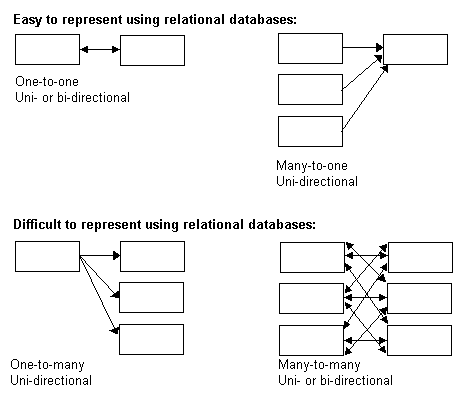
\includegraphics[scale=0.5]{pics/relations.jpg}
%			\caption{Отношения в базах данных} 
%			\label{pic:pic_name} % название для ссылок внутри кода
%		\end{center}
%	\end{figure}
	
	Для создания отношения Многие-ко-Многим используется аннотация ManyToMany. При этом создаётся промежуточная bridge-таблицы соотношений. Пример:
	\lstinputlisting[]{scripts/manytomany.java}
	
	Для создания отношения Многие-к-Одному используется аннотация ManyToOne. Пример:
	\lstinputlisting[]{scripts/manytoone.java}
	
	Один-ко-Многим это практически обратная связь, чтобы отобразить суть отношени объектов.
\end{enumerate}

\subsection{Миграция}
Миграции существуют для переноса изменений в моделях (добавление поля, удаление модели и т.д.) на структуру базы данных.
Сначала создадим новую миграцию.
\lstinputlisting[]{scripts/migration1.java}
В процессе создания генерируется SQL-скрипт на языке DDL на основе созданных классов и аннотаций: 
\lstinputlisting[style=SQL]{scripts/migsql.sql}

Затем применим текущую миграцию:
\lstinputlisting[]{scripts/migration2.java}

Увидим, что есть одна локальная и одна успешно применённая миграция.

\lstinputlisting[]{scripts/miginf.java}

По завершению миграции, база данных содержит все таблицы из схемы, а также таблицу db\_migrations, которая необходима для работы системы миграции.


\subsection{Заполнение данными}
Для заполнения тестовыми данными таблиц создадим отдельный класс:
\lstinputlisting[]{scripts/data.java}

\section{Выводы}
В данной работы было проведено знакомство с фреймворком Ebean для Java, позволяющим создавать ORM представление базы данных, миграциями моделей, а также с manage-командами для наполнения базы данных. Из достоинств фреймворка можно выделить
\begin{enumerate}
	\item Ускорение процесса изменения схемы базы данных;
	\item Возможность отслеживания схемы базы данных;
	\item Поддержка многими бэкендами(PostgreSQL, MySQL, SQLite);
	\item Возможность отката.
\end{enumerate}

ORM как раз и предназначен для инкапсуляции бизнес логики, но не на уровне СУБД, а на уровне приложения.
ORM дает много других приемуществ: валидация, кеширование, разделение прав доступа, миграции и много других готовых вещей, которые не нужно изобретать заново.
Использование ORM в проекте избавляет разработчика от необходимости работы с SQL и написания большого количества кода, часто однообразного и подверженного ошибкам. Весь генерируемый ORM код предположительно хорошо проверен и оптимизирован, поэтому не нужно в целом задумывается о его тестировании.
Однако при больших и тяжёлых запросах всё таки эффективнее использовать прямые SQL запросы.

\section{Дополнения}
\lstinputlisting[]{scripts/Departments.java}
\lstinputlisting[]{scripts/Doctors.java}
\lstinputlisting[]{scripts/Patients.java}
\lstinputlisting[]{scripts/Grants.java}
\lstinputlisting[]{scripts/Drugs.java}
\lstinputlisting[]{scripts/Diseases.java}
\lstinputlisting[]{scripts/Treatment.java}
\lstinputlisting[]{scripts/Services.java}
\lstinputlisting[]{scripts/Payments.java}
\lstinputlisting[]{scripts/DiseasesTypes.java}
\lstinputlisting[]{scripts/LoadExampleData.java}

\end{document}